\section{Methodology} \label{sec:methodology}
Next, we will delve into the details of the experimental setup.
We will discuss the data sources and their transformation, the creation of the graph database,
and the application of algorithms on the graph database.
The source code and result of this research is publicly available and can be found here:\\
\url{https://github.com/SiBergmann/gene_activity_in_lung_cancer}

\subsection{Data} \label{subsec:data}

Our study consists of two main datasets.
One includes healthy tissue data from the Genotype-Tissue Expression (GTEx) project,
and the other includes cancerous tissue data from the Cell Model Passport (CMP) project.
While these resources are widely used and well-established in research, they do have limitations in terms of their scope and coverage.
The GTEx dataset consists of only adult postmortem donor samples, with 2/3 of them between 50 and 69 years old and 2/3 being male~\cite{GTEX_modelannotation}.
The Cell Model Passport dataset contains data from donors who are predominantly male (60\%)
and have an age range that is biased towards older adults (50-69 years old)~\cite{CMP_modelannotation}.

The two datasets provide the foundation for our graph database, specifically for the gene nodes.
We aim to create a table with genes as rows,
where each row contains a unique Ensemble ID along with one value representing healthy TPM and another value representing cancerous TPM.
\\

% Genotype-Tissue Expression (GTEx) dataset
% TODO - K - i und j als numnber of genes und tissues oder als variable dafür?!
For the healthy tissue samples used in this study,
we utilized the $"$GTEx\_Analysis\_2017-06-05\_v8\_\newline
RNASeQCv1.1.9\_gene\_tpm$"$ dataset from the GTEx portal~\cite{gtex_download}.
The \textbf{GTEx portal} is a large-scale, publicly available resource for studying gene activity.
The Adult GTEx project aims to characterize the gene expression patterns in healthy tissues across different individuals,
providing valuable insights into the underlying biology of human development and disease.

The used dataset $A_{orig}$ is in a .gct file format that contains TPM values for 56,156 genes $i$ identified by
Ensemble ID as rows in 17,382 different tissues $j$ as columns (see~\cref{tab:gtex_table}.0).
The data was initially stored in a file in wide format where each tissue $j$ had its own column.
The TPM values for these tissues range between 0 and 747,400.
Since there are no missing values in the dataset, we did not need to handle any missing data.
To process this data into a suitable format, we employed the following steps:

\begin{enumerate}
    \item \textbf{Reshaping to long format:}
    We read the data from the original format in chunks of 3,000 rows at a time due to RAM capacity constraints.
    For each chunk of data, we transformed the columns for each tissue $j$ into individual rows,
    resulting in a dataset with three columns and 976.103.592 ($i * j$) rows (see~\cref{tab:gtex_table}.1).

    \item \textbf{Grouping by genes:}
    Once all chunks had been processed, we separated the combined dataset again for RAM reasons
    in new chunks of approximately 200 million rows.
    These chunks have been grouped by gene using an aggregate function that calculated
    both the sum $S_i$ and count $C_i$ of TPM values for each gene $i$ (see~\cref{tab:gtex_table}.2).

    \item \textbf{Calculating mean TPM:}
    To handle genes that had been split across multiple chunks,
    we performed a global aggregation on the genes of the sum of the dataset.
    Then we calculated the mean TPM value $M_i$ for each gene $i$ by dividing the sum $S_i$ by the count $C_i$
    of each observation (see~\cref{tab:gtex_table}.3).
\end{enumerate}

\begin{table}[h]
    \centering
    \resizebox{\textwidth}{!}{
    \begin{tabular}{|c|c|c|c|}
        \hline
        \textbf{0. Original Format} & \textbf{1. Reshaping to long format} & \textbf{2. Grouping by genes} & \textbf{3. Calculating mean TPM} \\
        \hline
        & & & \\[1mm] % adding more space to the row
        $\begin{aligned}
        i & : \text{number of genes} \\
        j & : \text{number of tissues} \\
        a_{ij} & : \text{TPM for gene } i \text{ in tissue } j
        \end{aligned}$ &

        $ A_{\text{long}} = (\text{Gen}_i, \text{Tissue}_j, a_{ij}) $ &
        $ A_{\text{agg}} = (\text{Gen}_i, S_i, C_i )$ &
        $ A_{\text{mean}} = (\text{Gen}_i, M_i )$ \\

        & & & \\[1mm] % adding more space to the row
        & & $ S_i = \sum_{j=1}^{j} a_{ij}, \quad C_i = \sum_{j=1}^{j} 1 $ &
        $ M_i = \frac{S_i}{C_i} $ \\

        & & & \\[1mm] % adding more space to the row

        $ A_{\text{orig}} = \begin{bmatrix}
            a_{11} & a_{12} & \dots & a_{1j} \\
            a_{21} & a_{22} & \dots & a_{2j} \\
            \vdots & \vdots & \ddots & \vdots \\
            a_{i1} & a_{i2} & \dots & a_{ij}
        \end{bmatrix} $ &

        $ A_{\text{long}} = \begin{bmatrix}
            \text{Gen}_1 & \text{Tissue}_1 & a_{11} \\
            \text{Gen}_1 & \text{Tissue}_2 & a_{12} \\
            \vdots & \vdots & \vdots \\
            \text{Gen}_i & \text{Tissue}_j & a_{ij}
        \end{bmatrix} $ &

        $ A_{\text{agg}} = \begin{bmatrix}
            \text{Gen}_1 & S_{1} & C_{1} \\
            \text{Gen}_2 & S_{2} & C_{2} \\
            \vdots & \vdots & \vdots \\
            \text{Gen}_i & S_{i} & C_{i} \\
        \end{bmatrix} $ &

        $ A_{\text{mean}} = \begin{bmatrix}
            \text{Gen}_1 & M_{1}\\
            \text{Gen}_2 & M_{2} \\
            \vdots & \vdots\\
            \text{Gen}_i & M_{i}\\
        \end{bmatrix} $ \\

        & & & \\[1mm] % adding more space to the row
        \hline
        & & & \\[1mm] % adding more space to the row

        % Example Matrix Representation
        $ A_{\text{orig}, i} = \begin{bmatrix}
            8.764 & 0.07187 & \dots & 3.215
        \end{bmatrix}$ &

        $ A_{\text{long}, i} = \begin{bmatrix}
            \text{ENSG...938} & \text{GTEX-111...} & 8.764 \\
            \text{ENSG...938} & \text{GTEX-112...} & 0.07187 \\
            \text{ENSG...938} & \text{GTEX-113...} & 3.215
        \end{bmatrix}$ &

        $ A_{\text{agg}, i} = \begin{bmatrix}
            \text{ENSG...938} & 12.051 & 3
        \end{bmatrix}$ &

        $ A_{\text{mean}, i} = \begin{bmatrix}
            \text{ENSG...938} & 4.017
        \end{bmatrix}$ \\

        & & & \\[1mm] % adding more space to the row
        \hline
    \end{tabular}
    }
    \caption{Data transformation pipeline for the GTEx dataset: Formulae and example data per gene}\label{tab:gtex_table}
\end{table}

The resulting dataset (see~\cref{fig:03_01_df_GTEX_healthy_mean}) with 56,156 genes $i$
and a mean TPM value $M_i$ was saved as a CSV file for further processing.\\

\begin{figure}[h]
    \centering
    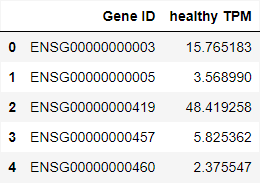
\includegraphics[height=\dfheight]{figures/03_01_GTEX_healthy_mean}
    \caption{Example data of processed Genotype-Tissue Expression dataset}
    \label{fig:03_01_df_GTEX_healthy_mean}
\end{figure}




% Cell Model Passport
For the analysis of gene activity in lung cancer, we utilized data from the \textbf{CMP project},
a comprehensive resource for studying cancer-related gene expression.
% TODO wirte more about The CMP project...

We obtained the dataset from the CMP portal~\cite{cmp_download} with the name \texttt{rnaseq\_all\_data\_20220624}.
This dataset contains data from the Sanger Institute and the Broad Institute and
consists of a file containing genes associated with diverse cancer types, including lung cancer.
Initially, the data was stored in long format with columns for IDs for genes, tissues, TPM values, and additional information.
% TODO J - Explain that its their own ID and not ENS ID
To focus on lung cancer-specific data, we loaded an additional file containing model annotations. \cite{cmp_tissue_models}
Then we filtered the CMP dataset to include only models from the annotation file with lung cancer as the cancer type.
% Todo more Details - what is the name fpor lung cancer? Small Cell Lung Carcinoma', Non-Small Cell Lung Carcinoma', Squamous Cell Lung Carcinoma'

The resulting dataset comprises 7,564,389 rows containing genes and tissues with associated TPM values for lung cancer.
Specifically, the dataset includes information on 37,262 unique genes across 203 distinct tissue types.
Notably, this dataset is free from missing values, and the TPM values span a range of 0 and 132,676.

To prepare the data for further processing, we performed the following steps:
\begin{enumerate}
    \item \textbf{Grouping by genes:} We grouped the dataset by genes to obtain a mean TPM value for every gene.
    This step involved aggregating the data by gene names, resulting in a new dataset with a mean TPM value for each gene.
    \item \textbf{Adding ENS ID:}
    The original dataset contained only CMP ID per gene but lacked the universal Ensembl ID required for matching genes across datasets.
    To address this limitation, we needed to add corresponding Ensembl IDs to our genes using their gene\_symbol.
    For this purpose we downloaded an Ensemble file from biomart~\cite{bio_marts},
    which contains the ENS ID and gene\_symbol.

    By analyzing the file, we encountered an issue where some gene\_symbols were not unique in the Ensemble file.
    To resolve this problem, we dropped all rows with duplicate gene\_symbols. %, which reduced the number of rows in the Ensemble file by a significant amount. % 10.605/48.311 rows
    We then merged the Ensemble table with our CMP data on gene\_symbols to retrieve the ENS IDs for each gene.

    \item \textbf{Removing missing ENS ID:} After merging the data, we found that 3,760 genes had no ENS ID associated with them.
    Since these genes were likely duplicates or did not exist in the Ensemble file,
    we removed them from our dataset to ensure consistency and accuracy of our analysis.
    % wie viele der missing data wären in den duplicate gewesen
\end{enumerate}
The resulting dataset~\ref{fig:03_01_df_CMP_cancer_mean} contains 33,502 genes with mean TPM values for lung cancer and was saved as a CSV file for further processing.

% TODO Table for CMP processing steps


\begin{figure}[h]
    \centering
    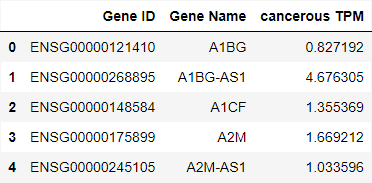
\includegraphics[height=\dfheight]{figures/03_01_CMP_cancer_mean}
    \caption{Example data of processed Cell Modell Passport dataset}
    \label{fig:03_01_df_CMP_cancer_mean}
\end{figure}



\subsection{Nodes and Edges} \label{subsec:nodes_and_edges}

As a next step we focus on describing how to create the base information for our advanced PPI Network.
The graph database contains gene and protein node types.
The Edges between the proteins build a classical PPI Network and are called Interactions. % mehr biologische Erklärung?
The second type of Edges, called Connections, are the Link between Proteins and Genes.
As Shown in the Figure~\ref{fig:03_02_Network}.
% TODO Wir machen das, weil …

\begin{figure}[h]
\centering
\includegraphics[width=0.8\textwidth]{figures/03_02_Network}
\caption{Schema of the Graph Database}
\label{fig:03_02_Network}
\end{figure}

For each of those 4 components we will create a table that will serve as base for creating the graph database.\\


For creating the \textbf{gene nodes} we need to use the preprocessed CMP and GTEx datasets,
which contain mean TPM values for cancerous and healthy genes.
We build the intersection of both datasets on their ENS ID to get a subset that only contains genes with TPM values for both conditions.
% filtering for genes that have a gene-protein connection
To fulfill our first objective~\ref{obj:delta_tpm},
we need to calculate a measure that captures significant changes between cancerous and healthy gene activity.
When examining the mean TPM values per dataset, we observe a right-skewed distribution, with most values close to zero
and a long tail extending towards higher values.
The cancerous TPM values vary from 0 to approximately 41.173, while the healthy TPM values range from 0 to around 36.200.



To normalize the TPM values from both datasets and enable better comparability, we perform a common log scaling between 0 and 1 for all TPM values combined.

\begin{equation}
\label{eq:tpm_normalization}
log\_norm(x) = \frac{\log(1 + x) - \log(1 + x_{min})}{\log(1 + x_{max}) - \log(1 + x_{min})}
\end{equation}

where $x_{\max}$ and $x_{\min}$ are the maximum and minimum TPM values across both datasets.
After applying the normalization, the distribution of the TPM values is more balanced, as shown in Figure~\ref{fig:03_02_normalized_tpm_both}.

\begin{figure}[h]
\minipage{0.45\textwidth}
    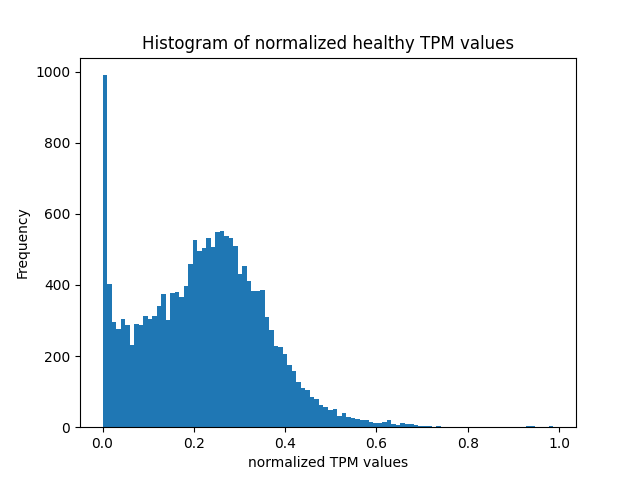
\includegraphics[width=\linewidth]{figures/03_02_normalized_gtex_tpm}
    \caption{Histogram of TPM Values of GTEx Dataset}
\endminipage
\hfill
\minipage{0.45\textwidth}
  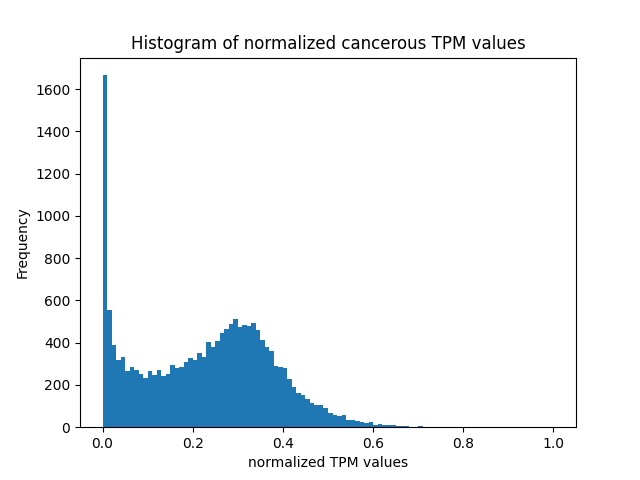
\includegraphics[width=\linewidth]{figures/03_02_normalized_cmp_tpm}
  \caption{Histogram of TPM Values of CMP Dataset}
\endminipage
\label{fig:03_02_normalized_tpm_both}
\end{figure}




Next, we calculate the difference between the normalized mean healthy and cancerous TPM values per gene
by subtracting the two values and call it $\Delta_{TPM}$.
The distribution of $\Delta_{TPM}$ values is shown in Figure~\ref{fig:03_02_delta_tpm}.

\begin{figure}[h]
\centering
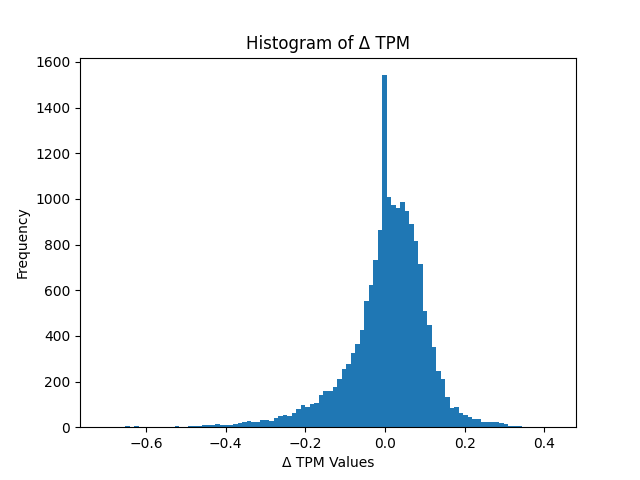
\includegraphics[width=0.5\textwidth]{figures/03_02_delta_tpm}
\caption{Distribution of $\Delta_{TPM}$ Values}
\label{fig:03_02_delta_tpm}
\end{figure}

We then define an $\Delta_{type}$ as either $increase$ or $decrease$, depending on whether the delta value is positive or negative.

As a final step for our first objective~\ref{obj:delta_tpm}, we need to determine if a change in gene activity is significant. % Doppelt
To do this, we use the z score measure, which calculates how many standard deviations a delta TPM value is away
from the mean of all delta TPM values.
The $z score$ is given by:

\begin{subequations}
    \begin{equation} \label{eq:z_score}
        z score (x) = \frac{x - {\mu}}{\sigma}
    \end{equation}
    \begin{equation}
        \text{where } \mu = \frac{1}{n} \sum_{i=1}^{n} x_i
        \label{eq:mean}
    \end{equation}
    \begin{equation}
        \text{where } \sigma = \sqrt{\frac{1}{n-1} \sum_{i=1}^{n} (x_i - \mu)^2}
        \label{eq:std}
    \end{equation}
\end{subequations}
% TODO check formular | mean(x) = and std(x) =

where $x$ is the delta TPM value, $\mu$ is the mean of all delta TPM values, $\sigma$ is the standard deviation of all delta TPM values,

We define a threshold of  $z score = 1.96$ to indicate significant changes in gene activity,
which corresponds to a confidence level of 95\% (p = 0.05).
Genes with delta TPM values exceeding this threshold will be flagged as $true$ in the $\Delta_{tpm} relevant$ column.

The resulting table contains 17.626 Gene Nodes as rows with their associated attributes,
including TPM values and derived metrics such as Delta TPM or Z-Score.
The head of the table is shown in Figure~\ref{fig:03_02_df_gene_nodes}.

\begin{figure}[h]
\centering
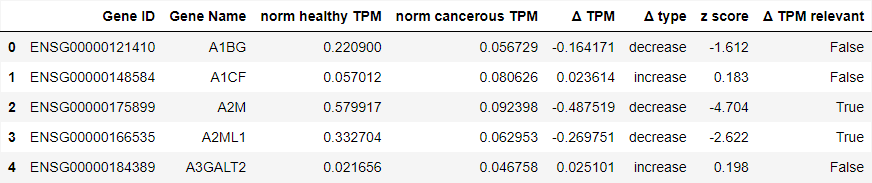
\includegraphics[height=\dfheight]{figures/03_02_gene_nodes}
\caption{Example data of Gene Nodes Table}
\label{fig:03_02_df_gene_nodes}
\end{figure}


% Gene Protein Edges
To construct the \textbf{gene-protein edges} we need a table that links the gene to the corresponding protein
which is translated from the transcript of this gene.
For this purpose we downloaded a file from biomart with Gene IDs and their Protein IDs. [LINK]
% The initial dataset comprised of XXX entries.
First we filtered for a subset (Intersection) to only include rows where the Ensembl ID for the gene matched an existing gene node
Since we have some genes without an entry for proteins, we need to drop them ; otherwise, there will not be an edge.

The final gene-protein edge table~\ref{fig:03_02_df_gene_protein_edges} features 101,731 rows as edges and two columns:
Ensembl ID for the gene and Ensembl ID for the protein translation.
The dataset highlights a key aspect of protein biology - one gene can be translated into multiple proteins.

\begin{figure}[h]
\centering
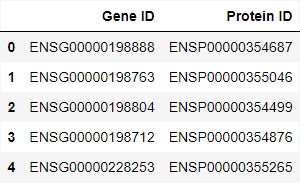
\includegraphics[height=\dfheight]{figures/03_02_gene_protein_edges}
\caption{Example data of Gene Protein Edges Table}
\label{fig:03_02_df_gene_protein_edges}
\end{figure}


% Proteins Nodes
We can generate the \textbf{protein nodes} from the gene-protein edges
since we only need a PPI for those proteins that are linked to our genes of interest.
To do this, we filter out the Gene colum from the previous file and check if there are any duplicate proteins.
Since there are no duplicate proteins our data indicates that every protein is uniquely translated by a single gene.
We do not need any additional attributes for these protein nodes because are focusing on the edges of this network.

The resulting table is a list of 101.731 unique Protein Ensembl IDs as shown in Figure~\ref{fig:03_02_df_protein_nodes}.
\begin{figure}[h]
\centering
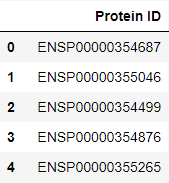
\includegraphics[height=\dfheight]{figures/03_02_protein_nodes}
\caption{Example data of Protein Nodes Table}
\label{fig:03_02_df_protein_nodes}
\end{figure}
\\

% protein protein edges
To create the \textbf{protein-protein edges} we download the String Database [LINK] with the information about the Protein-Protein Interaction.
We ensure that there are no duplicate entries.

The resulting file~\ref{fig:03_02_df_protein_edges} consists of 11.247.242 rows of protein-protein edges with a column for both protein IDs for the edge.
\begin{figure}[h]
\centering
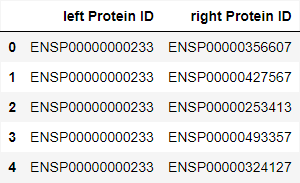
\includegraphics[height=\dfheight]{figures/03_02_protein_edges}
\caption{Example data of Protein-Protein Edges Table}
\label{fig:03_02_df_protein_edges}
\end{figure}




\subsection{Graph Database} \label{subsec:graph_database}
% Checked - all edges are created with 'match' statement
% todo check numbers of Protein Edges!! current number is only proteins directly on genes
% TODO Bezeichnung der IDs in Cypher Queries nochmal prüfen
% TODO check final version of the Cypher query for gene nodes with all attributes

% Intro
As we have created our base data models, our next objective~\ref{obj:graph_algorithm} is to create a graph database
that can be used to perform the PageRank algorithm as a graph algorithm.
With four huge datasets at our disposal, optimizing the generation of the database is crucial.
In this section, we describe the queries, called cypher queries, used to create and populate our graph database,
including information about creating indexes, constraints, relationships between nodes, and loading data into the database.\\


% PPI Network
To construct the \textbf{basic PPI network}, we need to create protein nodes and their interactions as edges.
To optimize query execution, we start with indexing the protein property $ID$.
Next we load the data (\ref{subsubsec:protein_nodes}~-~Protein nodes) as a list and then create the nodes in batches for efficient processing.
The graph database is populated with 104,235 protein nodes.

Since these nodes are used solely for connections between genes, no additional properties are required.
The cypher query for creating protein nodes is:

\begin{lstlisting}[language=Cypher, label={lst:protein_nodes}]
    CREATE (p:protein {id: 'Protein ID'})
\end{lstlisting}


We then create interaction edges by loading the saved data (\ref{subsubsec:protein_protein_edges}~-~Protein-protein edges)
as a list of protein tuples and searching for both protein nodes by their ID in the graph database.
The edges are created in batches for efficient processing, resulting in 11,247,242 interactions between protein nodes.

The cypher query for creating protein-protein edges is:

\begin{lstlisting}[language=Cypher, label={lst:protein_edges}]
    MATCH (s:protein{id:'left Protein ID'})
    MATCH (s:protein{id:'right Protein ID'})
    CREATE (s)-[:interaction]->(t)
\end{lstlisting}

We now have a complete PPI network in place.\\

% MATCH p=()-[r:interaction]->() RETURN p LIMIT 5
\begin{figure}[h]
    \centering
    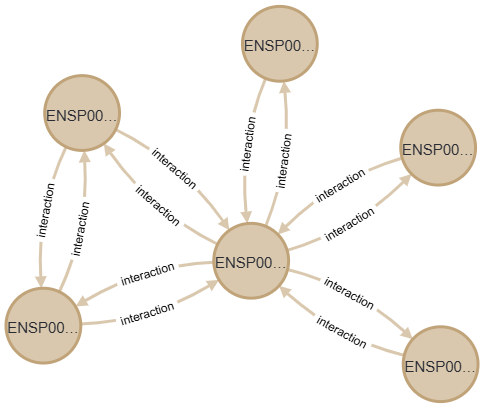
\includegraphics[width=0.35\textwidth]{figures/03_03_Basic_Network}
    \caption{Extract from the graph database setup showing example protein nodes and their interactions.}
    \label{fig:03_03_Basic_Network}
\end{figure}



%%%%%%%%%%%%%%%%%%%%%%%%%%%%%%%%%%%%%%%%%%%%%%%%%%%%%%%%%%%%%%%%%%%%%%%%%%%%%%%%%%%%%%%%%%%%%%%%%%%%%%%%%
% Extending the Network with Genes
Our actual focus is on the genes.
For constructing our \textbf{extended PPI network} with genes on the edges of the protein nodes, we need to connect them to the proteins.
To achieve this, we first create gene nodes with their associated attributes,
utilizing efficient data loading techniques to facilitate faster query execution.
Specifically, we implement an index on the gene property id to expedite querying,
load the data as a list, create nodes in batches to optimize processing,
and ultimately populate the graph database with 17,626 gene nodes.

The Cypher query employed for creating these gene nodes is:
\begin{lstlisting}[language=Cypher, label={lst:gene_nodes}]
    CREATE (p:gene {
            id: 'id',
            gene_name: 'gene_name',
            norm_healthy_tpm: 'norm_healthy_tpm',
            norm_cancerous_tpm: 'norm_cancerous_tpm',
            delta_tpm: 'delta_tpm',
            delta_type: 'delta_type',
            delta_tpm_relevant: 'delta_tpm_relevant'})
\end{lstlisting}

The genes in our network will be characterized by several properties:
$gene\_name$, $norm\_healthy\_tpm$, $norm\_cancerous\_tpm$, $delta\_tpm$, and $delta\_type$.


Among these, the calculation of $delta\_tpm\_relevant$ stands out as a pivotal factor in our analysis.
Although other attributes may be less relevant to our current investigation, they retain potential value for future tasks.

To model relationships between genes and proteins,
we establish connections between these nodes by loading gene-protein interaction data as a list of tuples.
This involves matching both gene and protein nodes based on their respective Ids,
and creating edges in batches to optimize processing efficiency.
The result is a comprehensive network of 101,731 connections between gene and protein nodes

The Cypher query for creating gene-protein connection edges is:
\begin{lstlisting}[language=Cypher, label={lst:gene_protein_edges}]
    MATCH (s:protein{id:'Protein ID'})
    MATCH (s:gene{id:'Gene ID'})
    CREATE (s)-[:connection]-(t)
\end{lstlisting}

% TODO Alternativ Verlinkung zu oben
\begin{figure}[h]
    \centering
    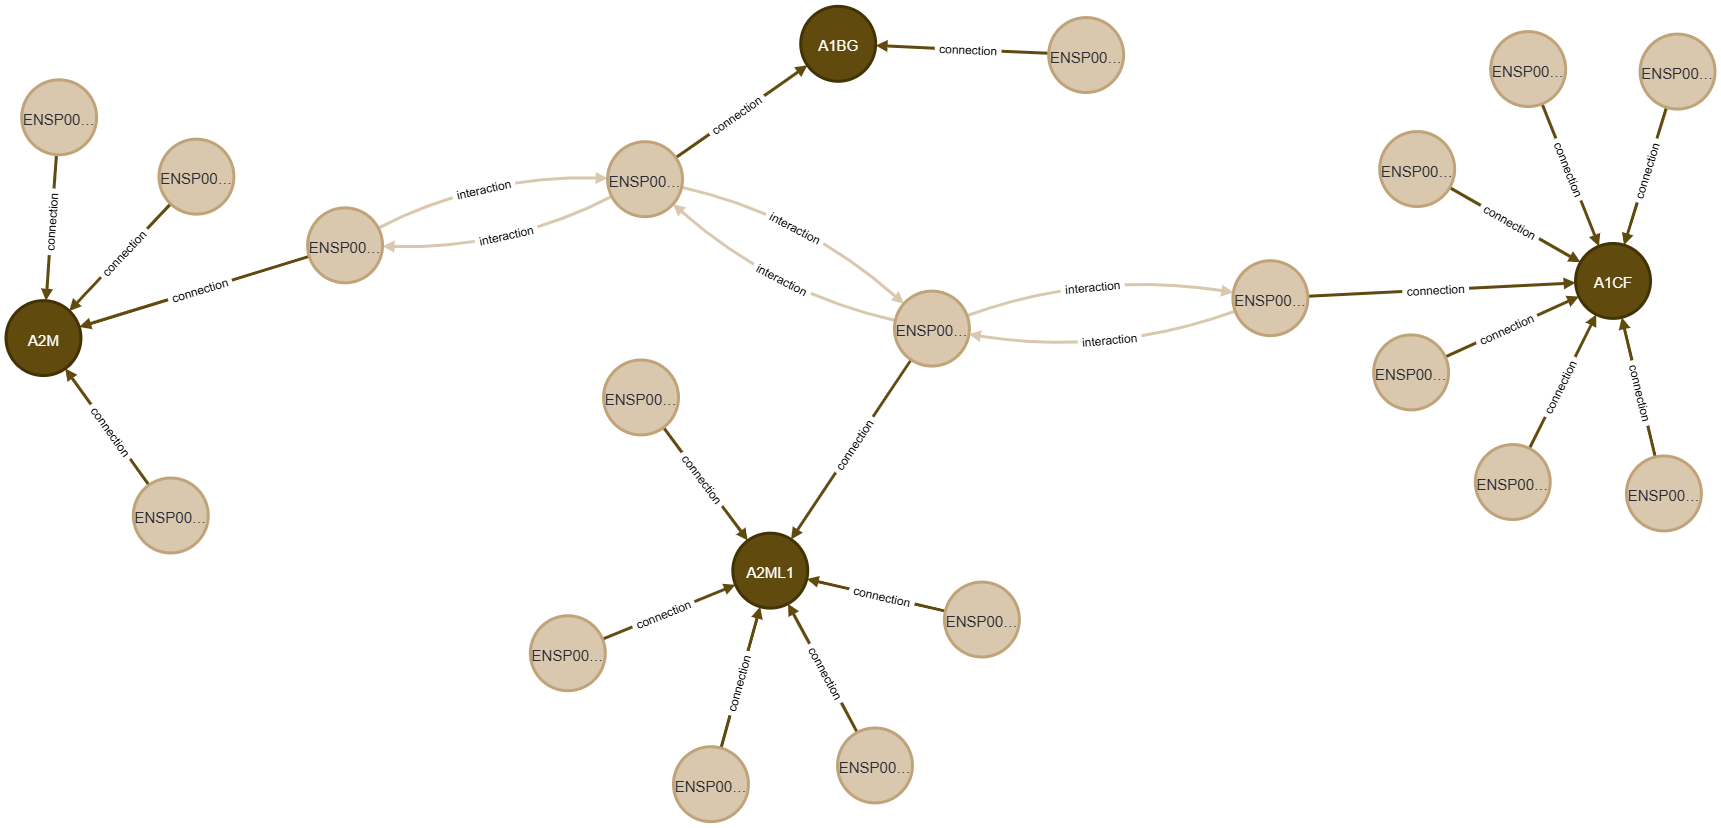
\includegraphics[width=1\textwidth]{figures/03_02_Network_2}
    \caption{Extract from the graph database setup ...}
    \label{fig:03_02_Network_2}
\end{figure}

Through the execution of these Cypher queries,
we are able to populate our graph database with the necessary nodes and edges to perform the PageRank algorithm.\\

\subsection{Applying PageRank Algorithm to Graph Database} \label{subsec:graph_database_algo}

As our final step for objective~\ref{obj:graph_algorithm},
we employ the PageRank algorithm to measure the importance of nodes within our graph database.
This algorithm is particularly well-suited for identifying genes that play a crucial role in the network,
enabling us to identify not only highly connected genes but also those with significant functional relevance.

For efficient computation and scalability,
we start with creating a projection of the entire graph prior to applying PageRank analysis to our large-scale graph database.

To perform the PageRank analysis, we use the following cypher query:
\begin{lstlisting}[language=Cypher, label={lst:pagerank}]
    CALL gds.pageRank.stream('gene_protein_graph')
    YIELD nodeId, score
    RETURN gds.util.asNode(nodeId).id AS Gene_ID,
           gds.util.asNode(nodeId).gene_name AS Gene_Name,
           score,
           gds.util.asNode(nodeId).Δ_TPM AS Δ_TPM,
           gds.util.asNode(nodeId).Δ_TPM_relevant AS Δ_TPM_relevant
    ORDER BY score DESC
\end{lstlisting}

This query returns a list of nodes, including genes and proteins, along with their respective PageRank scores.
We select the genes by filtering out the proteins from this list, and
further refined them to include only those exhibiting a significant change in gene activity,
indicated by the value for $\Delta_{TPM relevant}$.

The resulting subset of genes represents a group that has not only high connectivity
within the network but also exhibit a substantial difference in gene expression.\\



In conclusion, by successfully completing our \ref{obj:delta_tpm}. and \ref{obj:graph_algorithm} objective,
we have created the base data, established a graph database and performed the PageRank algorithm on our network.
This has allowed us to identify key genes within the network that exhibit both high connectivity
and significant changes in gene activity.
